\chapter{System Architecture}
This chapter contains an overview over the architecture of this project. Classes and Method sigantures
use the same notation as in the code, which follows Python PEP8.

\section{Description of Concept}

\subsection{Classes}
\textbf{Comment:} Please note, that valiable and attribute names may differ from the actual implementation
found in the code and may be abbreviated or use a different word, while still keeping the meaning of the 
original. This should not be an issue, as class names and method signatures are the same as in the code.

The keycomponents of this scirpt are the so called \emph{Backup Classes}:

\begin{itemize}
    \item \verb|Backup(ABC)|
    \item \verb|File_Backup(Backup)|
    \item \verb|File_Type_Backup(Backup)|
\end{itemize}

Each of those classes is contained in it's own file. By using inheritence, it is possible to 
use the \emph{strategy pattern}, which lets us use different implementations of a specific method
based on the object that calls the method.  In this case, the abstract class \emph{Backup} 
defines an abstract method \verb|backup(self) -> None| which is implemented in the subclasses 
according to their specific task. In the \verb|main.py| file, it is possible to call this method
all instances of classes that inherit from \emph{Backup}.

% Describe the use of factory pattern to create backup strategies

\subsection{Programflow}    % Discribe the behaviour of the program
The behaviour of the program is defined in the \emph{main.py} file. Is responsible for setting up
loggers and the argumentparser in their respective functions. It will provide a tkinter root object, which
can be used to attach GUI objects to, though this should not be done, as the root window will be withdrawn.
It is best to define further GUI windows in its own class and add objects to the main function as needed.

After setup, the programm allways follows predefined steps:

\begin{enumerate}
    \item Ask the user source and destination directories
    \item Create an instance of the Backup class. Which one it will be is dependant on the procedure the user wants to run
    \item Ask the user which filetypes they want to backup (this is optional and only done if the procedure requires it)
    \item Call the backup method. After this, the program terminates
\end{enumerate}

\section{Component Overview}

\begin{figure}[!ht]
    \centering
    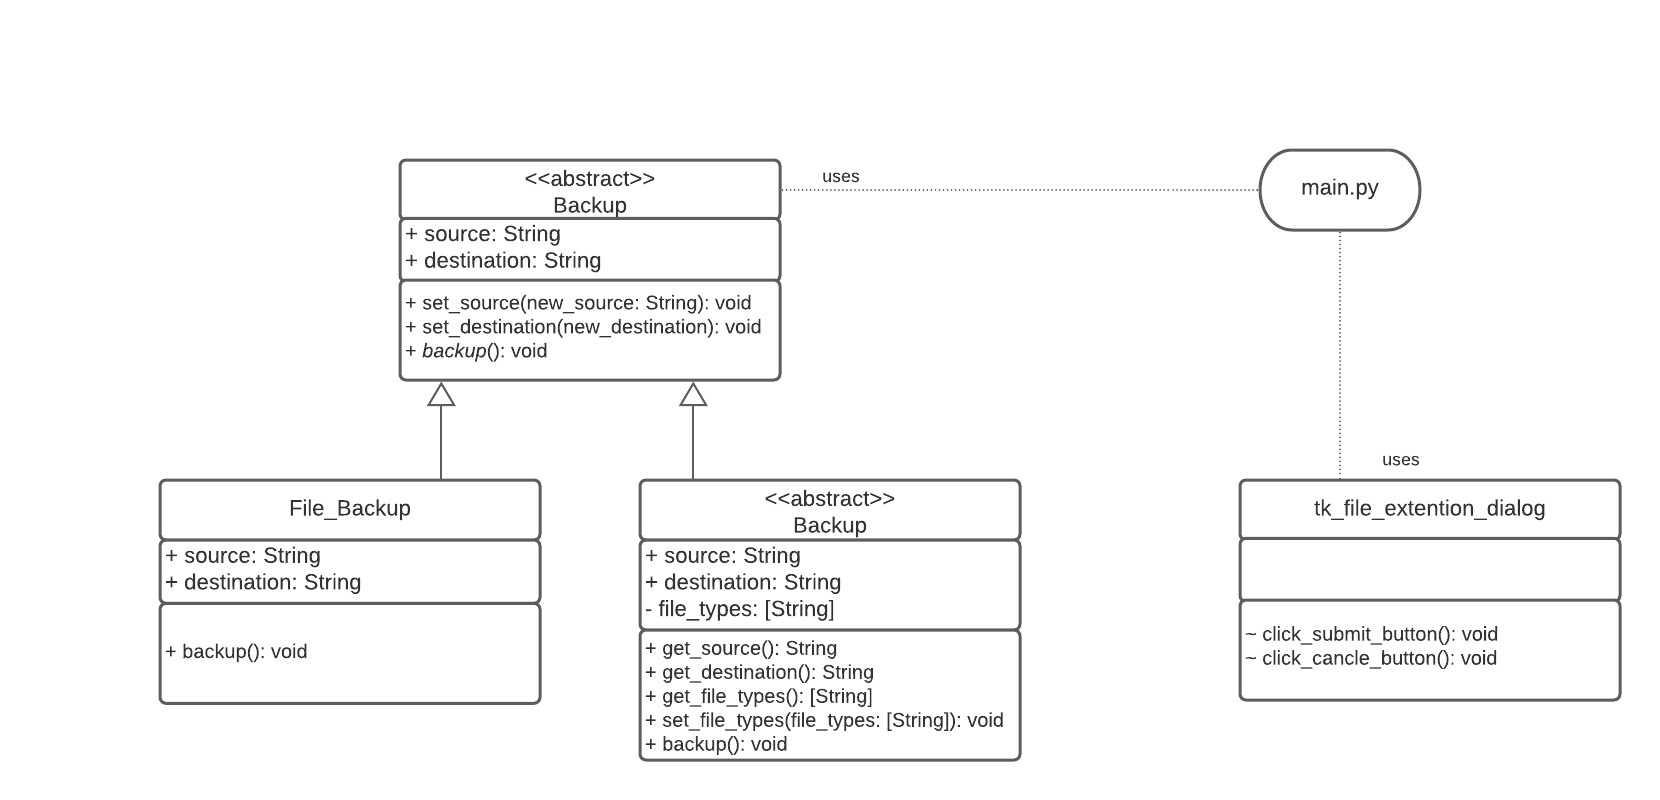
\includegraphics[scale=.5]{IMG/2021_12_21_UML_model.png}
    \caption
    {
        An UML overview over the classes used in the main script.
        On the left are all strategies used for backup. 
        The GUI class on the bottom right is not completely shown due to readability.
    }
    \label{fig:UML_class_view}
\end{figure}